% !TEX root = ../Dokumentation.tex
\subsection{Objekterkennung}
Die Objekterkennung hat das Ziel die richtigen Objekte zu erkennen und das genaue Positionieren des Fahrzeuges zu ermöglichen. Dabei wird die Containererkennung in zwei Teilaufgaben aufgeteilt: Die \glqq{Objekterkennung grob}\grqq{} ist für die Erkennung der richtigen Objekte mittels Farb- und Formerkennung zuständig. Die \glqq{Objekterkennung präzise}\grqq{} ist für das Positionieren des Fahrzeuges notwendig. Diese zwei Teilaufgaben werden separat angeschaut.
%
\subsubsection{Objekterkennung grob}
Die Aufgabe der \glqq{Objekterkennung grob}\grqq ist es, die aufzuladenden Container, kreuzenden Fahrzeuge und das Entleerungsbecken zu erkennen. Sobald ein solches Objekt erkannt wird, wird der zentrale Controller darüber informiert, damit die Informationen an die \glqq{Objekterkennung}\grqq{} präzise weitergegeben werden können.
\\[0.2cm]
\underline{\textbf{Container und Entleerungsbecken}}
\\[0.2cm]
\textbf{Funktionsbeschrieb}\\[0.2cm]
Bei der Container- und Entleerungsbeckenerkennung werden einerseits grüne und blaue Container und andererseits, im letzten Teil der Strecke, das Entleerungsbecken erkannt. Wird eines dieser Objekte erkannt, wird der Controller darüber informiert, damit sich das Fahrzeug auf das Auf- bzw. Abladen vorbereiten kann.
\\[0.2cm]
\textbf{Komponentenbeschrieb}\\[0.2cm]
Sobald die ersten Bilder mit der Kamera aufgenommen wurden, werden diese laufend aus dem Bilderpool abgefragt und untersucht. Dabei läuft die Erkennung von grünen und blauen Containern parallel ab. Erst sobald die Kreuzung zum zweiten Mal passiert wurde, wird auch nach dem Entleerungsbecken gesucht.
\begin{figure}[H]%Position festigen
\centering
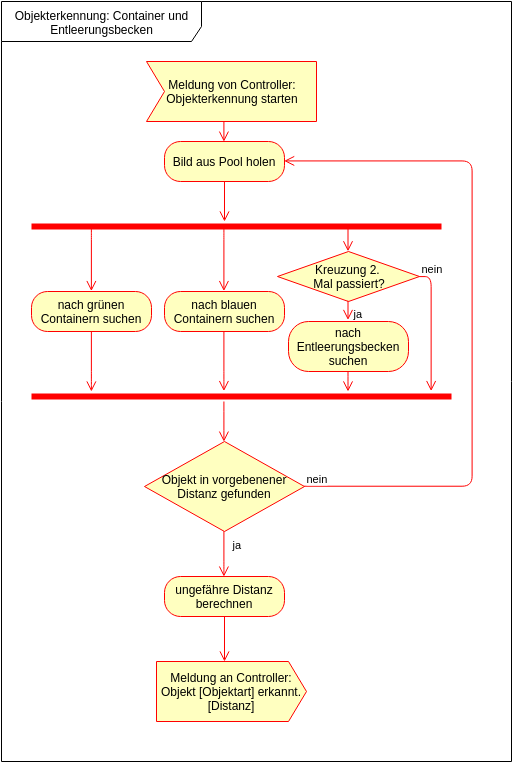
\includegraphics[width=0.6\textwidth]{03_Loesungskonzept/pictures/objekterkennung_containers.png}
\caption{Aktivitätendiagramm Obkjekterkennung: Container und Entleerungsbecken}
\label{fig:activityContainer}
\end{figure}
\newpage
Die Erkennung läuft dabei immer gleich ab. Als erstes wird das Bild mit OpenCV nach der entsprechenden Farbe gefiltert. Sprich: Es wird nur nach Grün-, Blau- und Weisstönen gesucht. Anschliessend werden mit Hilfe einer Konturerkennung störende und falsche Objekte entfernt. Mit der Höhe dieser Objekte kann dann ausgerechnet werden, wie weit das Objekt  noch entfernt ist. Diese Distanzberechnung liefert nur ein ungefähres Ergebnis. Ist das Objekt zu weit entfernt, wird der zentrale Controller nicht informiert. Ansonsten wird eine Meldung an den Controller gesendet, welche die Objektart und Distanz enthält.
\\[0.2cm]
\textbf{Begründung}\\[0.2cm]
Da der Blickwinkel auf die Container durch die Kurven variieren kann, wäre es wenig sinnvoll die Konturerkennung vor der Farberkennung durchzuführen. Es bestehen zu viele Möglichkeiten, dass ein störendes Objekt als Container oder Entleerungsbecken identifiert werden könnte. Dadurch, dass zuerst nach Farben gefiltert wird, können bereits viele falsche Objekte ausgeschlossen werden. \\
OpenCV stellt Methoden zur Verfügung, mit welcher ein ganzer Bereich mit Farbwerten im HSV-Format angegeben werden kann. Das bedeutet, dass auch bei unterschiedlichen Lichtverhältnissen die Farbtöne korrekt erfasst werden können.
\\[0.2cm]
\textbf{Testergenisse} \\[0.2cm]
Die Containererkennung wurde bereits soweit getestet, dass grüne und blaue Container bis auf eine bewusst eingeschränkte Distanz erkannt werden können. 
\begin{figure}[H]%Position festigen
\centering
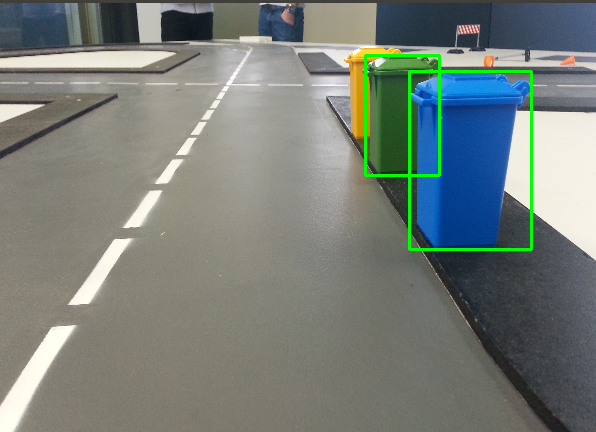
\includegraphics[width=0.6\textwidth]{03_Loesungskonzept/pictures/containererkennung_blau_gruen.png}
\caption{erfolgreicher Testversuch}
\label{fig:erfolgreicher Testversuch}
\end{figure}
Auch bei aufgenommenen Bildern, welche gleichfarbige Container mit unterschiedlichen Lichtverhältnissen zeigen, konnten die Container korrekt erkannt werden:
\begin{figure}[H]%Position festigen
\centering
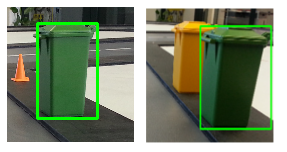
\includegraphics[width=0.6\textwidth]{03_Loesungskonzept/pictures/containererkennung_div_brightness.png}
\caption{unterschiedliche Helligkeiten}
\label{fig:unterschiedliche Helligkeiten}
\end{figure} \\
Bei den Testversuchen wurden jedoch auch Probleme und Risiken aufgedeckt. Falls zum Beispiel im Hintergrund ein Objekt steht, welches eine grüne oder blaue Farbe hat und dessen Masse einem Container entsprechen könnten, kann es zu einer Fehlerkennung kommen. Folgendes Bild zeigt einen solchen Fall:
\begin{figure}[H]%Position festigen
\centering
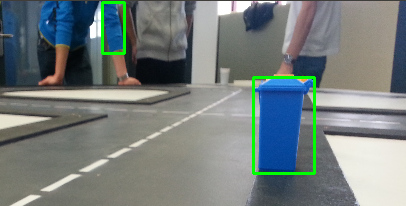
\includegraphics[width=0.6\textwidth]{03_Loesungskonzept/pictures/objekterkennung_blau_fehl.png}
\caption{fehlerhafter Testversuch}
\label{fig:fehlerhafter Testversuch}
\end{figure} \\
Um solche Fälle möglichst zu vermeiden, wird versucht den abzusuchenden Bereich einzuschränken, sodass nur solche Bildbereiche untersucht werden, wo sich auch wirklich ein Container befinden könnte. 
\\[0.2cm]
\underline{\textbf{Rechtsvortritt}}
\\[0.2cm]
\textbf{Funktionsbeschrieb}\\[0.2cm]
Falls sich an der Kreuzung ein gegnerisches Fahrzeug von rechts nähert, hat dieses gemäss Aufgabenstellung Vortritt. Die Objekterkennung muss ein solches Fahrzeug erkennen und den Controller darüber informieren, damit das Fahrzeug gestoppt wird.
\\[0.2cm]
\textbf{Komponentenbeschrieb}\\[0.2cm]
Sobald die Objekterkennung vom Controller informiert wird, dass das Fahrzeug gleich an der Kreuzung ankommen wird, wird Ausschau nach einem gegnerischen Fahrzeug auf der von rechtskommenden Spur gehalten. Wird ein Fahrzeug erkannt, wird dies dem Controller gemeldet. Der Vorgang wird wiederholt, bis das Fahrzeug nicht mehr im Bereich liegt. Nachdem dies geschehen ist, wird wieder der Controller informiert, damit das Fahrzeug weiterfahren kann.
\begin{figure}[H]%Position festigen
\centering
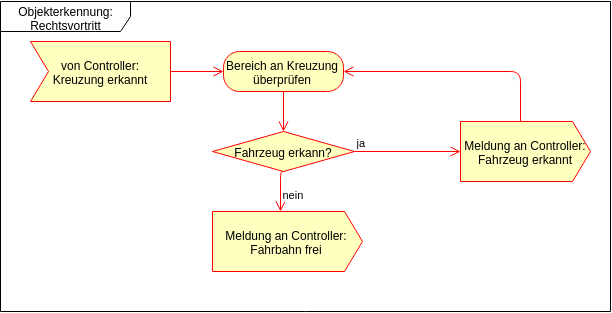
\includegraphics[width=0.8\textwidth]{03_Loesungskonzept/pictures/objekterkennung_rechtsvortritt.png}
\caption{Aktivitätendiagramm Obkjekterkennung: Rechtsvortritt}
\label{fig:activityRechtsvortritt}
\end{figure} \\
\newpage
Da nicht nur angehalten werden muss, wenn ein gegenerisches Fahrzeug an der Kreuzun steht, sondern auch, wenn es sich von rechts nähert, muss der zu überprüfende Bereich eine gewisse Grösse haben. Der ungefähre Bereich, welcher abgesucht werden soll, ist in der folgenden Grafik markiert:
\begin{figure}[H]%Position festigen
\centering
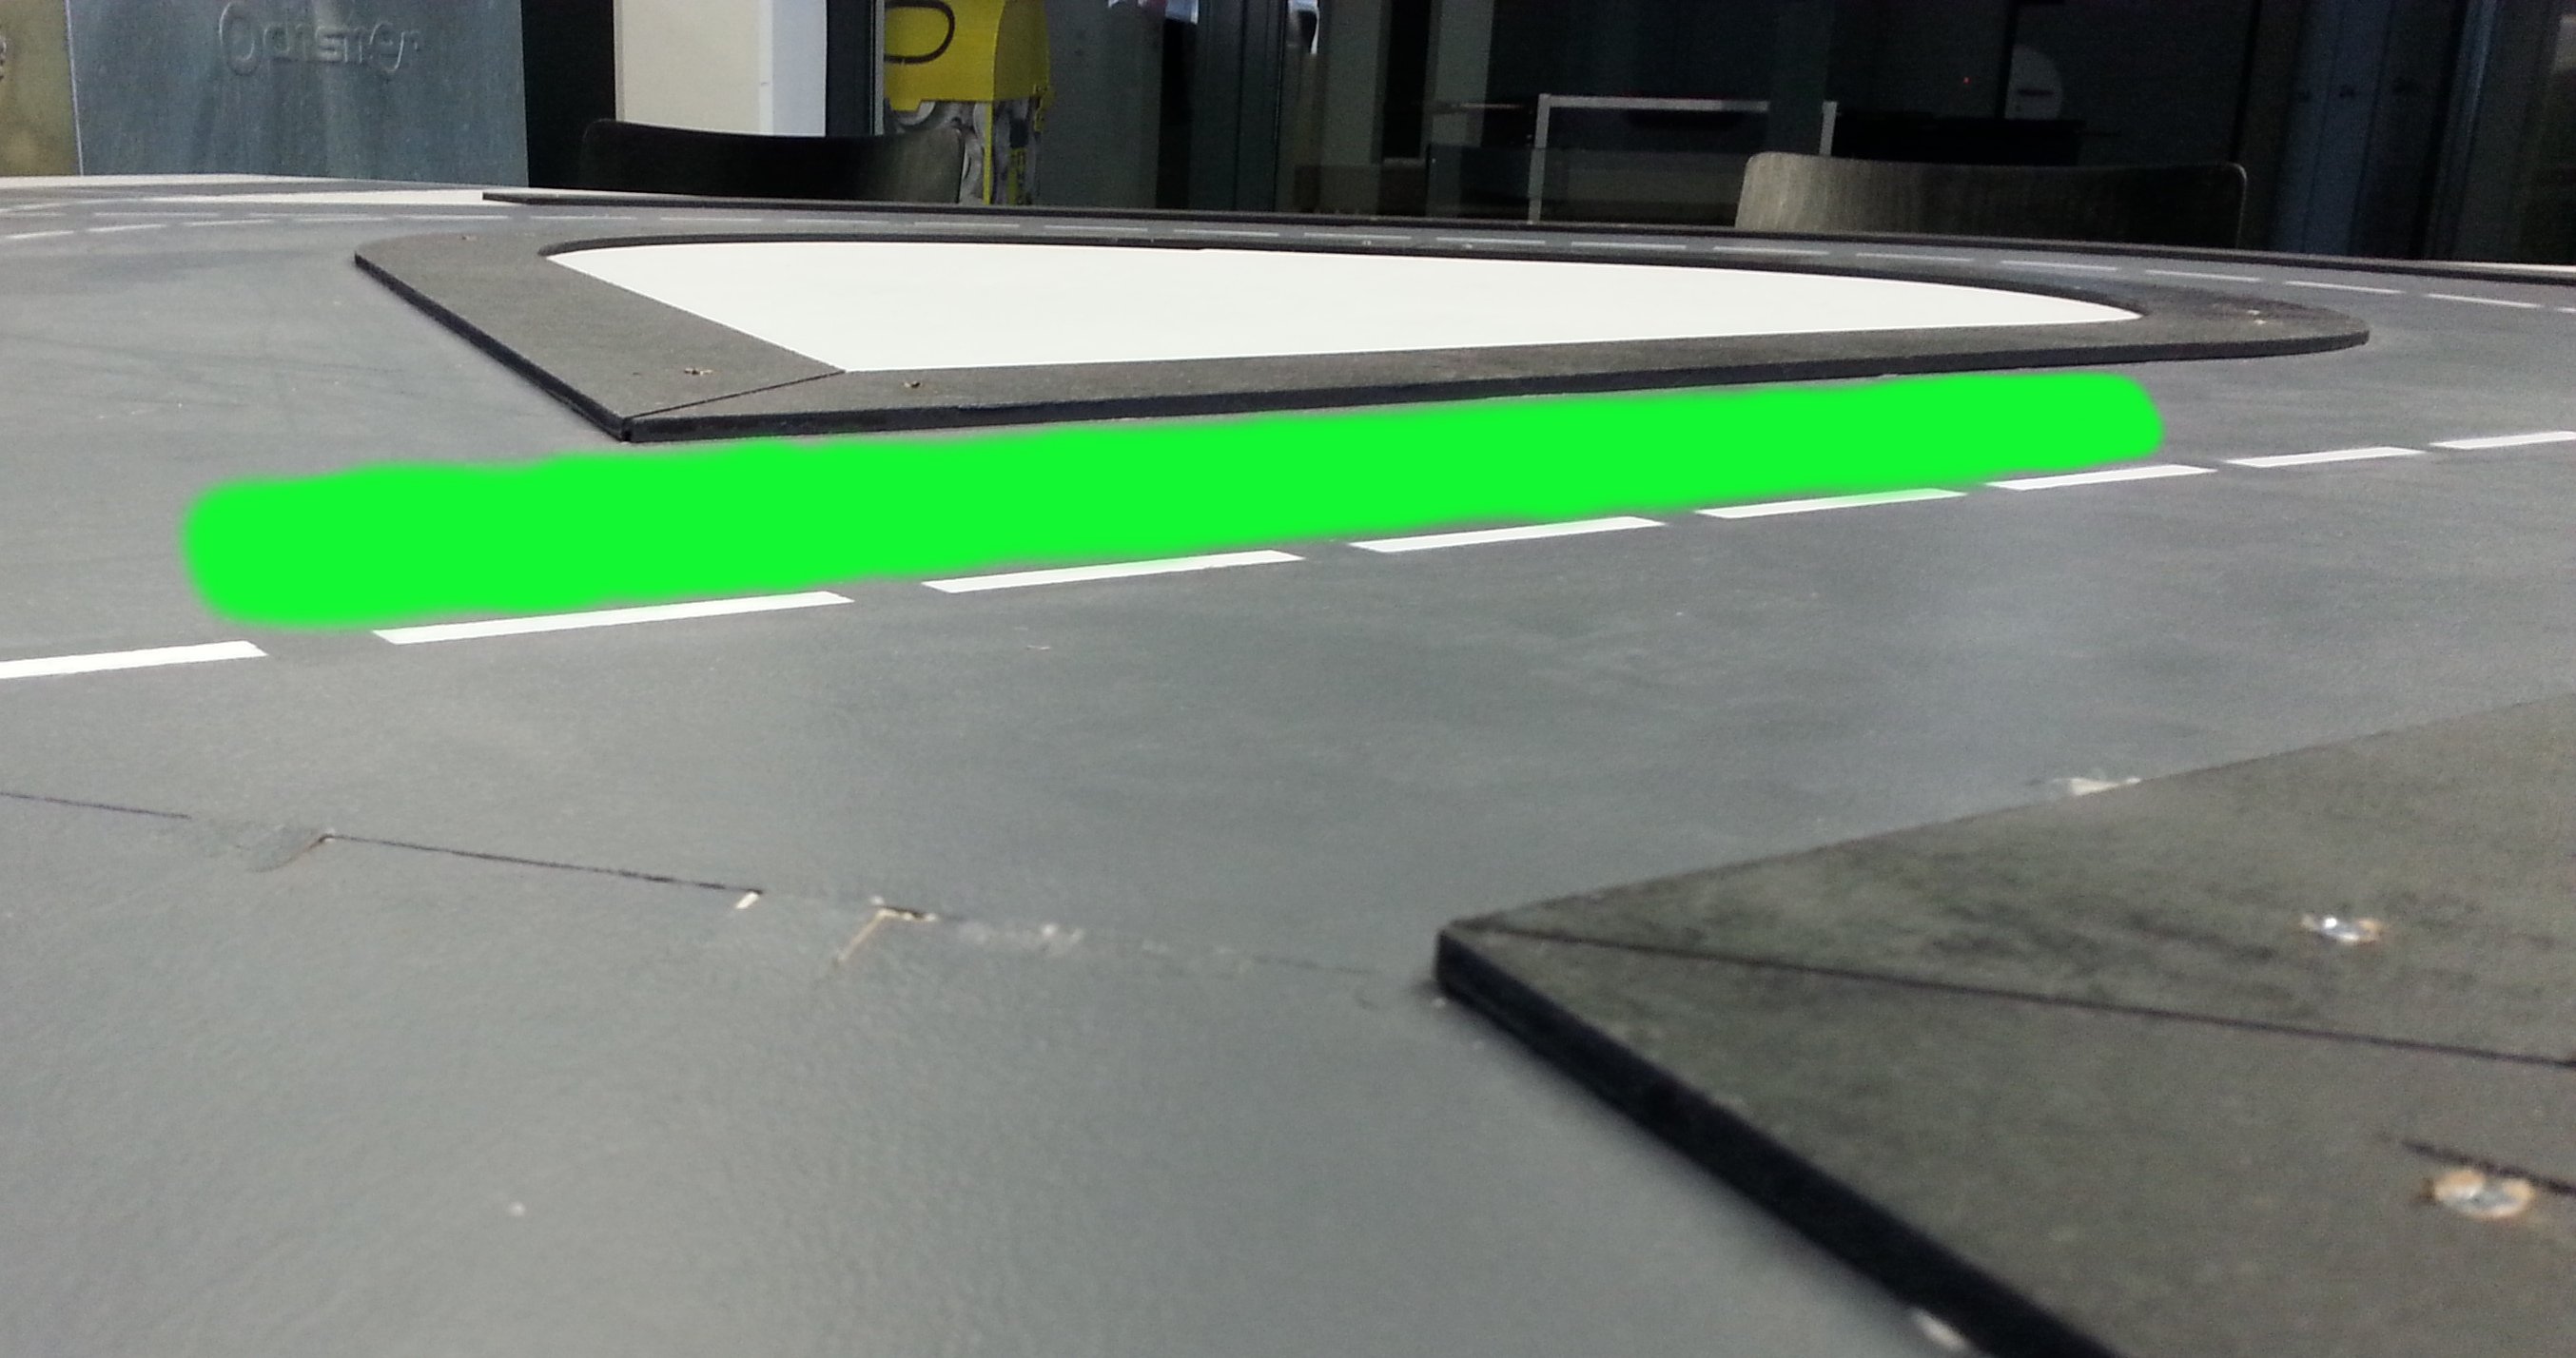
\includegraphics[width=0.6\textwidth]{03_Loesungskonzept/pictures/rechtsvortritt_bereich.jpg}
\caption{Abgedeckter Bereich beim Rechtsvortritt}
\label{fig:bereichRechtsvortritt}
\end{figure}
\\
\textbf{Begründung}\\[0.2cm]
Bei der Vortrittserkennung kann nicht nach Farben oder Konturen gesucht werden, da keine Angaben vorhanden sind, wie das gegnerische Fahrzeug aussieht. Daher ist es nötig, dass erkennt werden kann, ob ein definierter Strassenabschnitt verdeckt ist oder nicht. Falls der Abschnitt verdeckt ist, heisst das, dass sich ein Fahrzeug darauf befindet, welches Vortritt hat.
\subsubsection{Objekterkennung präzise}
\underline{\textbf{Containererkennung}}\\[0.2cm]
\textbf{Funktionsbeschrieb}\\[0.2cm]
Die präzise Containererkennung wird für das genaue Stoppen des Fahrzeuges gebraucht. Dieses Modul gibt den Trigger zum Anhalten.\\[0.2cm]
\textbf{Komponentenbeschrieb}\\[0.2cm]
Die Containererkennung wird mit Hilfe von Distanzsensoren realisiert. Dafür sind Infrarot-Distanzmesser oder Infrarot-Reflexkoppler vorgesehen. Diese werden auf der rechten Seite des Fahrzeuges befestigt. Sobald ein Objekt in der Nähe ist, ändert sich der Spannungswert, was einer Distanzänderung gleichkommt. 
\begin{figure} [H]
	\centering
	\includegraphics[width=0.35\textwidth]{03_Loesungskonzept/pictures/InfrarotContainererkennung.png}
	\caption{Beispielhafte Containererkennung mit einem Infrarotsensor}
\end{figure}
\textbf{Begründung}\\[0.2cm]
Die Positionierung mit einem Infrarotsensor ist die ideale Lösung. Sie ist einfach zu realisieren im Vergleich zu einer Kamera oder einem Farbesensor und präziserer als ein Ultraschallsensor.\\[0.2cm]
\textbf{Testergebnisse}\\[0.2cm]
Für die Ermittlung des besten Sensors wurde ein Ultraschall und Infrarotsensor als Funktionsmuster getestet. Der relativ grosse \glqq{Empfangswinkel}\grqq, welcher der Ultraschallsensor aufweist, ist in dieser Anwendung nicht gewollt. Der Infrarotsensor ist diesbezüglich besser. Dieser ist zwar lichtempfindlich, jedoch sollte dieses Problem gelöst werden können.\\[0.2cm]
%
\underline{\textbf{Rechtsvortritt}} \\[0.2cm]
\textbf{Funktionsbeschrieb}\\[0.2cm]
Die \glqq{Rechtsvortritterkennung detailliert}\grqq{} hat die Aufgabe das Fahrzeug vor einer Kollision mit einem zweiten Fahrzeug zu bewahren. Wenn rechts oder vor dem Fahrzeug etwas im Weg ist, soll das Fahrzeug anhalten.\\[0.2cm]
\textbf{Komponentenbeschrieb}\\[0.2cm]
\begin{figure} [H]
	\centering
	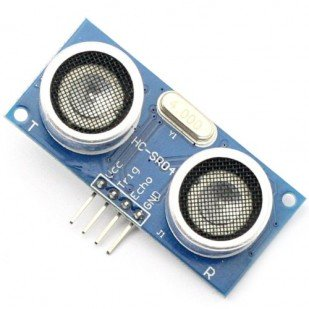
\includegraphics[width=0.23\textwidth]{03_Loesungskonzept/pictures/ultraschallsensor.png}
	\caption{Getesteter Ultraschallsensor (Quelle: www.generationrobots.com)}
	%http://www.generationrobots.com/2653-large_default/ultraschallsensor-hc-sr04.jpg
\end{figure}
Diese Aufgabe wird mit einem Ultraschallsensor gelöst. \\[0.2cm]
\textbf{Begründung}\\[0.2cm]
Ein Ultraschallsensor ist für unter fünf Franken zu haben und erfüllt mit seinem grossen Abstrahlwinkel und seiner Reichweite die geforderten Bedingungen. Zudem ist die Anbindung an das Freedomboard gut möglich.\\[0.2cm]
\textbf{Testergebnisse}\\[0.2cm]
Der Ultraschallsensor wurde bereits erfolgreich an das Freedomboard angeschlossen und  ausgewertet. Die Anbindung wurde mit Hilfe einer Anleitung von mcuoneclipse.com realisiert. Die Distanzauswertung funktionierte bei dem Test relativ genau ($\approx \pm $ 1cm).\\[0.2cm]
%
\underline{\textbf{Entleerungbecken Erkennung}} \\[0.2cm]
\textbf{Funktionsbeschrieb}\\[0.2cm]
Damit das Schüttgut im Entleerungsbecken entleert werden kann, muss das Entleerungsbecken richtig detektiert werden können. \\[0.2cm]
\textbf{Komponentenbeschrieb}\\[0.2cm]
Die Container und Fahrbahnerkennung benötigen bereits Sensoren. Dies wären der Flexsensor und der Infrarotsensor. Für die Detektion des Entleerungsbehälters ist kein weiterer Sensor mehr nötig. Die Detektion ist mit beiden Sensoren möglich. Bei Tests mit den beiden Sensoren wird sich zeigen, welcher dieser beiden besser geeignet ist.\\[0.2cm]
\textbf{Begründung}\\[0.2cm]
Die Einsparung von Sensoren entlastet das Budget und spart zusätzlichen Implementierungsaufwand.\\[0.2cm]